\section{Experiments}

It is now time to investigate, how the two efficient algorithms that
we derived in the previous section behave on real world datasets,
both in the context of maximum likelihood estimation as well as
in a Bayesian setting.
In order to do so, we selected three benchmark datasets in advance
that will be used to compare both algorithms to each other as
well as to the baseline uniform sampling procedure, where each
sample is simply selected with equal probability.

It is important to emphasize, that the datasets used in the evaluation
are not a result of cherry picking: We selected the same datasets
as \cite{on-coresets} as well as \cite{coresets-strengthened}
in order to be comparable to other works in the field, without
testing in advance if our algorithms look good on them or not.

Finally, we note that all of the following experiments were
implemented in Python and executed on an
AMD Ryzen 7 2700x processor with 8 cores of 3.7GHz clock speed
and 16GB of RAM.
The code for all the experiments is open source and can be
found publicly accessible on Github.\footnote{
    \url{https://github.com/cxan96/efficient-probit-regression}
}

\subsection{Datasets}

The datasets that are used in the empirical evaluation of our
algorithms are called Covertype\footnote{
    \url{https://archive.ics.uci.edu/ml/datasets/Covertype}
}, Kddcup\footnote{
    \url{https://kdd.ics.uci.edu/databases/kddcup99/kddcup99.html}
} and Webspam\footnote{
    \url{https://www.csie.ntu.edu.tw/\~cjlin/libsvmtools/datasets/binary.html\#webspam}
} and are
all publicly available.

The Covertype dataset consists of $n=581012$ observations of 30x30m
forest patches of wilderness areas located in the
Roosevelt National Forest of Northern Colorado, USA.
The task is to predict the so called covertype of each of these
patches, i.e. the dominant tree species, based on $d=54$
observed features. There are seven distinct tree species that
appear in the dataset, so we have a multiclass problem. To transform
the problem into a binary classification problem that can be
subjected to a probit analysis, we adapted the task to distinguish the
tree species "Lodgepole Pine" from the other six species, thus
obtaining a balanced problem of $49\%$ positive vs $51\%$ negative
observations.
As an additional preprocessing step, all continuous features of the
dataset were scaled to have a mean of zero as well as unit variance.
In addition, an intercept column of all ones was appended to the data.

The Webspam datasets consists of $n=350000$ observations of
web pages, that can either be classified as spam or no spam, based
on the occurence of 254 distinct words on the web page.
$61\%$ of the observations in the dataset are labeled as spam
and the other $39\%$ are labeled as no spam. The task is to predict,
whether a given web page is spam or not.
The features consist of binary $0/1$ observations that indicate, if
a given word is present on a web page or not.
In a preprocessing step, words that are never present
in the dataset were removed, as well
as words that are only present on a single web page.
After preprocessing, the dataset that is subjected to the
experiments consists of $d=128$ binary features.
An intercept column of all ones was appended to the Webspam dataset
as well.

The Kddcup dataset consists of $n=494021$ observations of network
connections, where the task is to predict if a connection is
"good" or "bad", i.e. to distinguish, whether a hacker tries
to gain unauthorized
access to a network or whether someone tries to establish a
normal connection.
$80\%$ of the connections in the dataset are "bad" and the other
$20\%$ are "good" connections.
In a preprocessing step, $d=33$ continuous features
were retained from the data and scaled to a mean of zero and
unit variance. Just like the other datasets, an intercept column
of all ones was appended to the Kddcup data as well.


\begin{table*}[ht!]
    \centering
    \begin{tabular}{ | l| r| r| r| r|}
        \hline
        \textbf{Dataset} & $\mathbf{n}$ & $\mathbf{d}$ \\ \hline
        Covertype        & $581\,012$   & $54$         \\ \hline
        Kddcup           & $494\,021$   & $33$         \\ \hline
        Webspam          & $350\,000$   & $128$        \\ \hline
    \end{tabular}
    \caption{Dimensions of the benchmark datasets under study. The
        values of $d$ do not include the intercept column, which was
        always added during the analysis.}
    \label{tab:datasets}
\end{table*}

\begin{figure}[ht!]
    \centering
    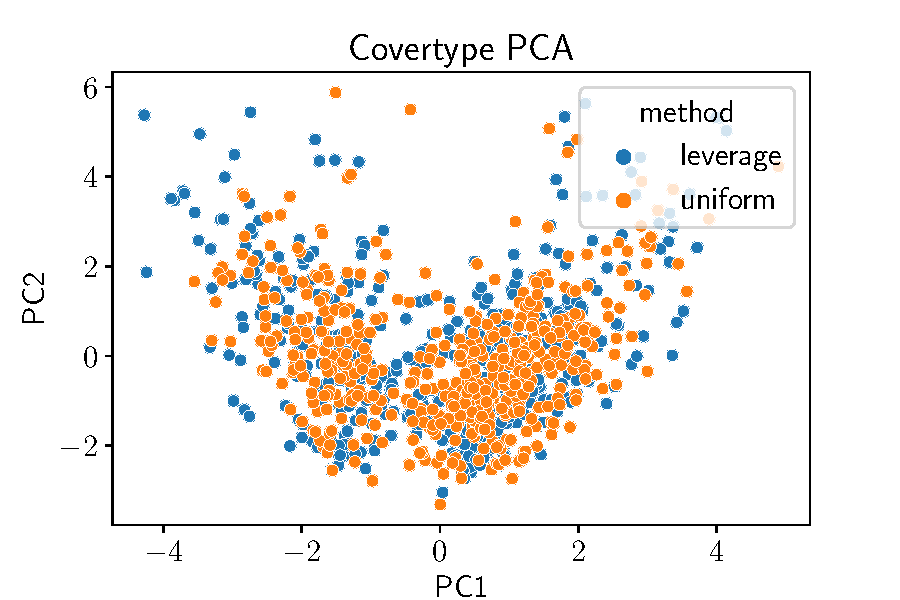
\includegraphics[width=.49\linewidth]{figures/covertype_pca.pdf}
    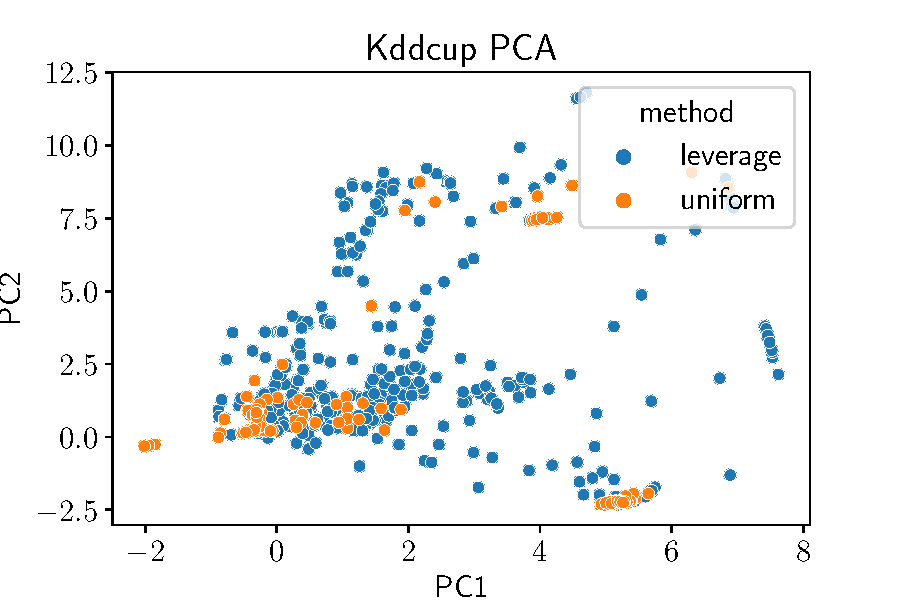
\includegraphics[width=.49\linewidth]{figures/kddcup_pca.pdf}
    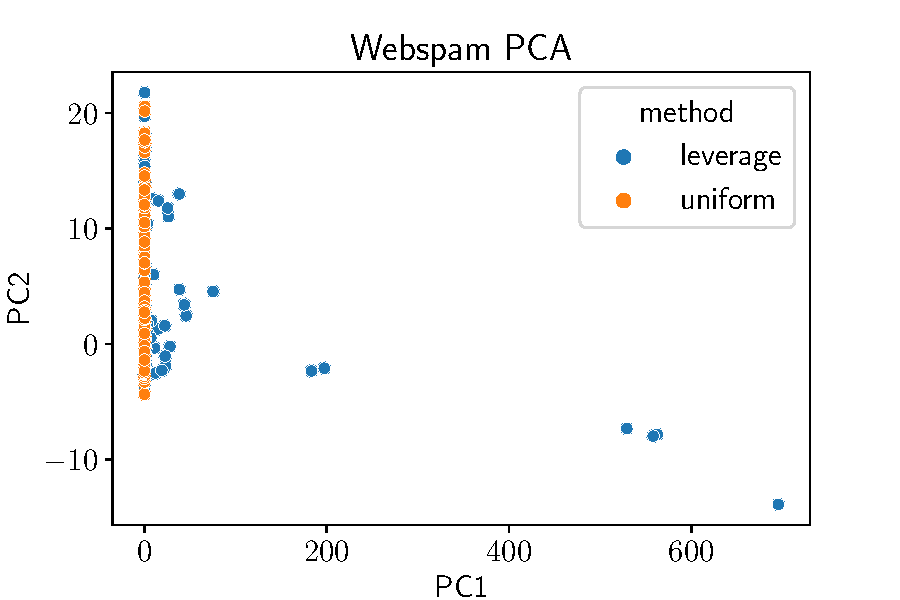
\includegraphics[width=.49\linewidth]{figures/webspam_pca.pdf}
    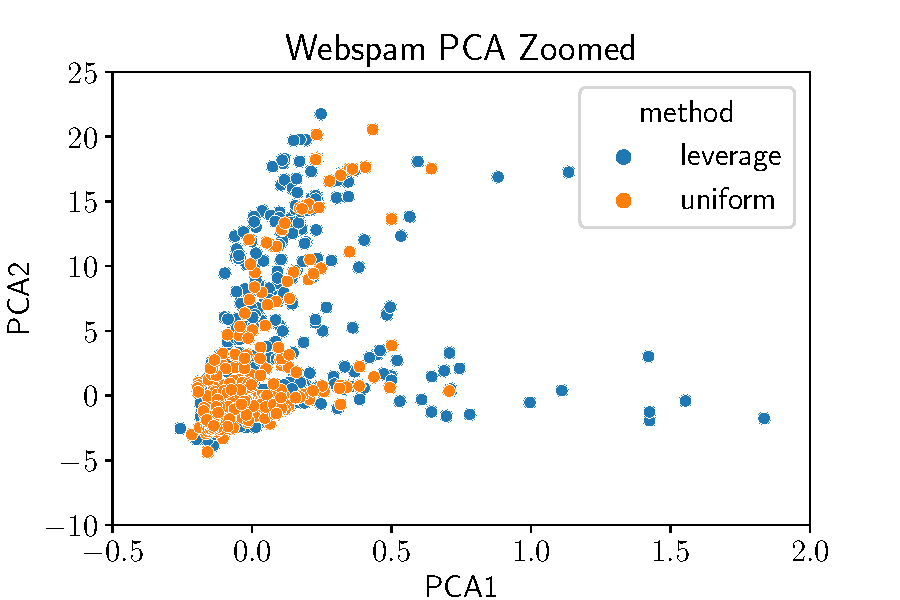
\includegraphics[width=.49\linewidth]{figures/webspam_pca_zoomed.pdf}
    \caption{The datasets are compared by projecting the datapoints
        onto the first two principal components and then drawing
        a random sample of 500 points (a) uniformly and (b) proportionally to the
        statistical leverage scores of the original data.}
    \label{fig:dataset-comparison}
\end{figure}

\begin{figure}[ht!]
    \centering
    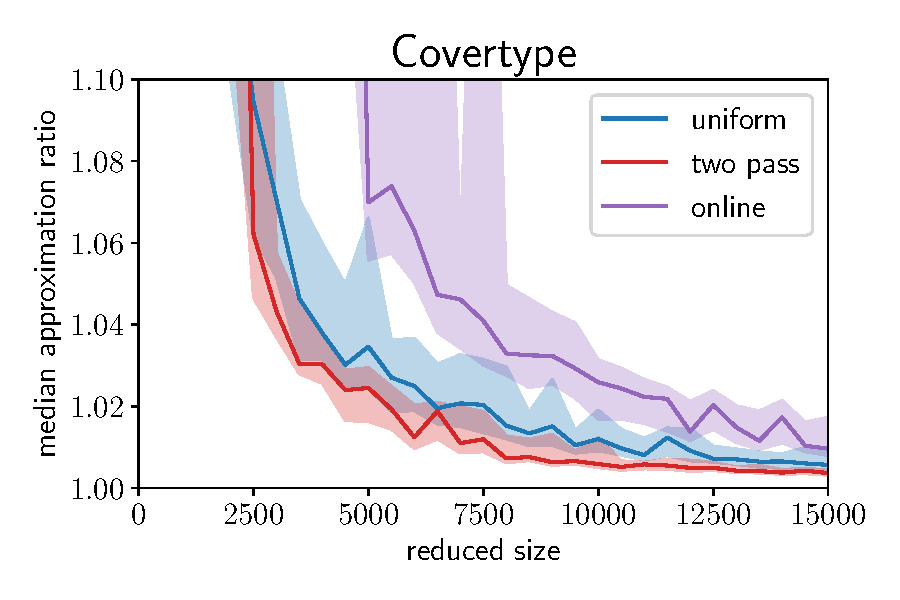
\includegraphics[width=.49\linewidth]{figures/covertype_ratio_plot.pdf}
    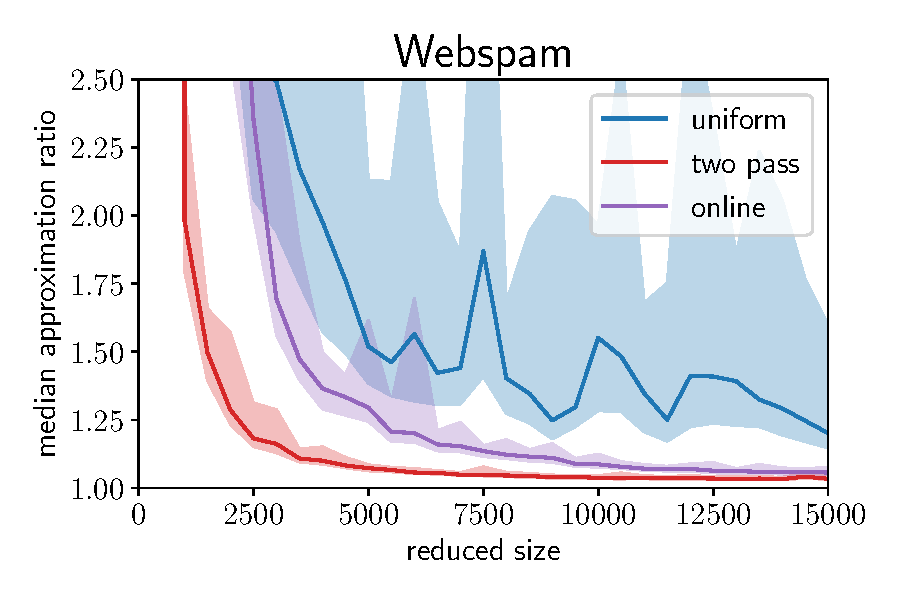
\includegraphics[width=.49\linewidth]{figures/webspam_ratio_plot.pdf}
    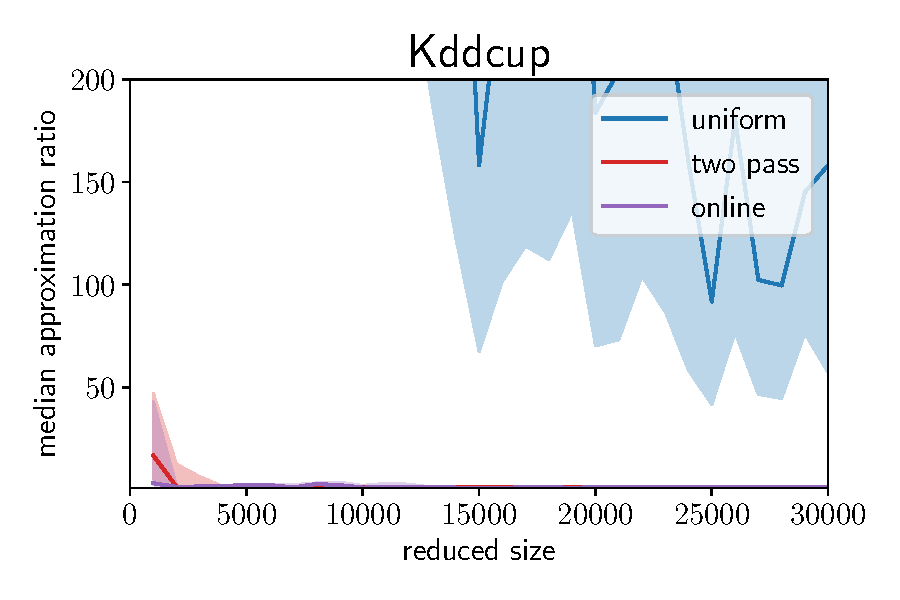
\includegraphics[width=.49\linewidth]{figures/kddcup_ratio_plot.pdf}
    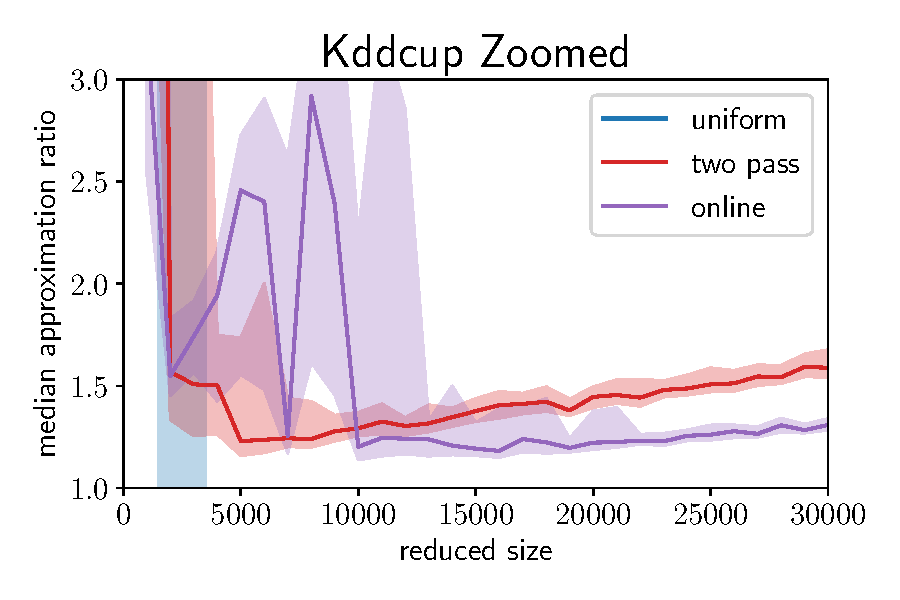
\includegraphics[width=.49\linewidth]{figures/kddcup_ratio_plot_zoomed.pdf}
    \caption{TODO.}
    \label{fig:ratio-plots}
\end{figure}